%%%%%%%%%%%%%%%%%%%%%%%%%%%%%%%%%%%%%%%%%%%%%%%%%%%%%%%%%%%%%%%%%%%%%%%%%%%%%%%
%  Cross-Layer Auditing Protocol: Eliminating Integrity Conflicts
%  in AI-Generated Content Provenance
%  IEEE Conference Paper — Final Draft with Figures
%%%%%%%%%%%%%%%%%%%%%%%%%%%%%%%%%%%%%%%%%%%%%%%%%%%%%%%%%%%%%%%%%%%%%%%%%%%%%%%
\documentclass[conference]{IEEEtran}
\usepackage{cite}
\usepackage{amsmath,amssymb,amsfonts}
\usepackage{algorithmic}
\usepackage{graphicx}
\usepackage{textcomp}
\usepackage{xcolor}
\usepackage{booktabs}
\usepackage{multirow}
\usepackage{array}
\usepackage{hyperref}
\usepackage{tikz}
\usepackage{flushend}

\usetikzlibrary{shapes,arrows,positioning,fit,backgrounds}

\hyphenation{}

\begin{document}

\title{Cross-Layer Auditing Protocol: Eliminating Integrity Conflicts
       in AI-Generated Content Provenance}

\author{\IEEEauthorblockN{Anonymous Authors}
\IEEEauthorblockA{Cross-Layer Auditing Protocol Research Team\\
Email: \{clap-research\}@example.com}}

\maketitle

\begin{abstract}
The proliferation of AI-generated images has created an unprecedented
digital trust crisis, demanding reliable provenance mechanisms to
distinguish synthetic from authentic content.
Existing solutions fall into two disjoint categories: metadata-based
signing frameworks such as the Coalition for Content Provenance and
Authenticity (C2PA) standard, and content-based invisible watermarking
techniques.
However, these two layers operate independently, creating an
\textit{integrity conflict} vulnerability: an adversary can construct a
malicious file whose C2PA metadata passes verification while its embedded
watermark tells a contradictory story, or vice versa, rendering single-layer
verification insufficient.

We present the Cross-Layer Auditing Protocol (CLAP), a unified provenance
framework that jointly evaluates C2PA metadata signatures and DWT-domain
blind watermarks through a formal decision matrix.
We define the \texttt{.aig} (AI-Generated) binary container format as the
first reference implementation, bundling an Ed25519-signed C2PA manifest
with a WebP-encoded image payload carrying a Haar-wavelet QIM watermark
whose payload is cryptographically bound to the manifest itself.

Our experimental evaluation on an Apple Silicon M-series platform
demonstrates a \textbf{100\% detection rate} across four representative
attack scenarios—signature stripping, C2PA spoofing, watermark overwriting,
and integrity conflict construction.
The complete cross-layer audit completes within 94.6\,ms at
$1024{\times}1024$ resolution, with a fixed metadata overhead of
approximately 930\,bytes (${<}10\%$ for resolutions above
$512{\times}512$).
To the best of our knowledge, CLAP is the first framework to unify
metadata-level signatures and content-level watermarks within a single
cross-layer auditing protocol, systematically eliminating the integrity
conflict attack surface.
\end{abstract}

\section{Introduction}

The rapid advancement of generative artificial intelligence (AI) has
democratised the creation of photorealistic images at an unprecedented
scale.  Tools such as Stable Diffusion, DALL-E, and Midjourney now
produce synthetic imagery that is often indistinguishable from authentic
photographs to the human eye.
While this technology unlocks creative potential across industries, it
simultaneously erodes the foundational trust upon which digital media
ecosystems rely.
Malicious actors exploit generative models to produce convincing
disinformation, fabricated evidence, and fraudulent identity documents,
threatening domains ranging from journalism and legal proceedings to
national security.
The urgency of establishing \textit{provable provenance}—the ability to
cryptographically trace a piece of content back to its origin and verify
the integrity of that chain—has never been greater.

Two broad categories of technical countermeasures have emerged to address
this challenge.
The first category, \textbf{metadata-based provenance}, attaches
cryptographic signatures to content at creation time.
The C2PA specification~\cite{c2pa_spec} represents the most prominent
industry effort in this direction, defining a manifest structure that
records the generating device, software agent, edit history, and other
contextual metadata, all wrapped in an Ed25519 or ECDSA digital
signature~\cite{rosenthol2022c2pa, c2pa_trust, parson2023c2pa}.
Major camera manufacturers and Adobe have adopted C2PA to establish
hardware-rooted authenticity chains~\cite{adobe_content_credentials,
leica_m11_content_credentials}.

The second category, \textbf{content-based watermarking}, embeds
imperceptible signals directly into the pixel domain of an image.
These techniques range from spatial-domain least-significant-bit (LSB)
methods to robust frequency-domain schemes employing Discrete Cosine
Transform (DCT), Discrete Wavelet Transform (DWT), or Singular Value
Decomposition (SVD)~\cite{cox2007digital, fang2020deep,
zhang2023robust_dwt}.
Recent research has explored deep-learning-based watermarking using
encoder–decoder architectures that jointly optimise imperceptibility and
robustness against common image processing operations~\cite{zhu2018hidden,
luo2020distortion_agnostic}.

Despite significant progress in both directions, these two layers have
evolved largely in isolation, creating a dangerous security gap that we
term the \textbf{Integrity Conflict} (IC) vulnerability.
In current practice, a C2PA verifier checks only the metadata signature
without examining the image content, while a watermark detector operates
solely on pixels without consulting the provenance manifest.
An adversary can exploit this decoupling to construct files where the
metadata and the content tell contradictory stories.
For instance, an attacker can strip the C2PA manifest from an
AI-generated image while retaining the watermark, or forge a C2PA
signature claiming ``authentic photograph'' while the embedded watermark
identifies the image as AI-generated.
Neither a pure-C2PA nor a pure-watermark verifier can detect both attacks
simultaneously.
Parsons~\cite{parsons2023integrity} first identified the conceptual
possibility of such layer-disagreement attacks but did not propose a
systematic protocol-level defence.

In this paper, we propose the \textbf{Cross-Layer Auditing Protocol}
(CLAP), a unified framework that eliminates the integrity conflict
vulnerability by jointly evaluating metadata signatures and content
watermarks within a single, cryptographically coherent decision procedure.
The core insight of CLAP is that the C2PA manifest and the invisible
watermark must not be treated as independent evidence streams; rather,
they must be \textit{cross-referenced} such that any discrepancy between
them is automatically detected and flagged.
We realise this principle through three architectural components:
(i)~the \texttt{.aig} binary container format, which physically bundles
the C2PA manifest, its Ed25519 signature, and the watermarked image
payload into a single verifiable unit;
(ii)~a cryptographic binding mechanism wherein the watermark payload is
a SHA-256 digest of the canonical C2PA manifest, stored as a signed
assertion within the manifest itself; and
(iii)~a formal \textit{audit decision matrix} that maps the four possible
combinations of (C2PA verification, watermark detection) to authoritative
verdicts.

Our principal contributions are as follows:
\begin{enumerate}
    \item \textbf{Protocol Design:} We formalise the Cross-Layer Auditing
    Protocol (CLAP), the first provenance framework that jointly verifies
    metadata-level C2PA signatures and content-level DWT watermarks
    through a decision matrix, systematically closing the integrity
    conflict attack surface.
    \item \textbf{Format Specification:} We define the \texttt{.aig}
    binary container format, a concrete reference implementation that
    bundles generation provenance, an Ed25519-signed C2PA manifest, a
    DWT-QIM watermark, and a WebP image payload into a single,
    self-verifying file.
    \item \textbf{Security Validation:} We implement four representative
    attacks—signature stripping, C2PA spoofing, watermark overwriting, and
    integrity conflict construction—and demonstrate that CLAP achieves a
    \textbf{100\% detection rate}, whereas single-layer schemes miss at
    least two attack types each.
    \item \textbf{Performance Characterisation:} We provide a comprehensive
    benchmark across three image resolutions ($256{\times}256$,
    $512{\times}512$, $1024{\times}1024$), showing that a full CLAP audit
    completes within $94.6$\,ms at the highest resolution, with a fixed
    metadata overhead of ${\sim}930$\,bytes.
\end{enumerate}

The remainder of this paper is organised as follows.
Section~II surveys related work in metadata-based provenance,
content-based watermarking, and hybrid approaches.
Section~III details the CLAP architecture, the \texttt{.aig} format
specification, the audit decision matrix, and the underlying
cryptographic and watermarking primitives.
Section~IV presents our experimental evaluation, covering attack
detection rates, latency benchmarks, file overhead analysis, and
multi-dimensional comparison with baseline schemes.
Section~V concludes with a summary of contributions, a candid discussion
of limitations, and directions for future work.

\section{Related Work}

\subsection{Metadata-Based Provenance}

The Coalition for Content Provenance and Authenticity (C2PA) specification,
jointly developed by Adobe, Arm, Intel, Microsoft, and Truepic,
establishes an end-to-end provenance framework wherein content creators
cryptographically sign a manifest describing the origin and edit history
of a digital asset~\cite{c2pa_spec}.
Rosenthol et al.~\cite{rosenthol2022c2pa} provide a detailed technical
overview of the C2PA architecture, including the claim–assertion–signature
data model and the role of trust lists in establishing signer identity.
The specification leverages existing cryptographic standards—Ed25519
and ECDSA for signing, X.509 for certificate chains—to ensure
interoperability with established public key infrastructure.

Industry adoption has accelerated, with Adobe integrating C2PA Content
Credentials into Photoshop and Lightroom~\cite{adobe_content_credentials},
Leica embedding C2PA signing directly in the M11 camera
firmware~\cite{leica_m11_content_credentials}, and the Content Authenticity
Initiative (CAI) promoting open-source verification
tooling~\cite{cai_opensource}.
However, Parsons~\cite{parsons2023integrity} critically observes that
C2PA's security guarantees are \textit{metadata-scoped}: the signature
attests to the integrity of the manifest, but the binding between the
manifest and the actual image content is only as strong as the hash stored
in the \texttt{c2pa.hash.data} assertion.
An attacker who strips or replaces the metadata wrapper entirely
can distribute the naked image, which will pass no C2PA verification
yet may still circulate as ``authentic'' in contexts where verification
is not mandatory.

\subsection{Content-Based Watermarking}

Digital watermarking embeds a covert signal into the content itself,
ensuring that provenance information survives format conversion, metadata
stripping, and screenshot-based redistribution.
Classical approaches operate in the frequency domain.
Cox et al.~\cite{cox2007digital} pioneered spread-spectrum watermarking in
the DCT domain, demonstrating robustness against JPEG compression.
Subsequent work shifted to the Discrete Wavelet Transform (DWT), which
offers multi-resolution decomposition better aligned with the human visual
system and modern compression pipelines~\cite{barni2003improved_dwt,
zhang2023robust_dwt}.

Quantisation Index Modulation (QIM), introduced by Chen and
Wornell~\cite{chen2001qim}, provides a capacity-achieving framework for
blind watermarking by modulating the host signal according to the message
bit to be embedded.
Recent research explores the robustness–imperceptibility–capacity
trade-off through adaptive embedding strengths, error-correction coding,
and perceptual models~\cite{fang2020deep, luo2020distortion_agnostic}.
Deep-learning-based methods~\cite{zhu2018hidden, tancik2020stegastamp}
train encoder–decoder networks to jointly optimise embedding and
extraction, achieving state-of-the-art robustness against a range of
distortions at the cost of model complexity and the need for large
training datasets.

A fundamental limitation of watermarking-only approaches, however, is
that they provide no mechanism for authenticating \textit{who} created the
content or under what circumstances.
A watermark can signal that an image was AI-generated, but cannot
cryptographically bind that signal to a specific device, software version,
or signer identity.
Furthermore, watermark detectors typically output a confidence score
rather than a binary verifiable proof, making them less suitable for
high-assurance applications such as legal evidence or press photography.

\subsection{Hybrid Approaches and Remaining Gaps}

Recognising the complementary strengths of metadata and watermarking,
several efforts have explored their combination.
The two-path verification model, informally practised by some content
authentication platforms, runs C2PA verification and watermark detection
independently and reports both results to a human analyst.
However, as Parsons~\cite{parsons2023integrity} argues, this approach
merely presents two independent pieces of evidence without any
\textit{protocol-level correlation} between them; it remains vulnerable to
the integrity conflict scenario where an attacker ensures one layer passes
while the other is compromised.

Recent proposals by Balan et al.~\cite{balan2023ekila} and
Golaszewski et al.~\cite{golaszewski2026verifying} explore embedding a provenance
identifier within the watermark that references the C2PA manifest, but
these designs stop short of a formal decision procedure that
deterministically adjudicates the trustworthiness of the content based on
the joint state of both layers.
The IETF's Media Origin and Provenance working group~\cite{ietf_mops}
has also acknowledged the need for ``binding across layers'' as an open
research problem.

To the best of our knowledge, \textbf{no existing method provides a
protocol-level framework that unifies metadata signatures and content
watermarks within a single cryptographic audit procedure, where the
watermark payload is itself a signed assertion of the C2PA manifest and
a formal decision matrix eliminates ambiguity in the joint verification
outcome}.  This is precisely the gap that CLAP fills.

\section{Methodology}

\subsection{System Overview}

CLAP is organised as a three-layer architecture, illustrated in
Figure~\ref{fig:architecture}:

\begin{enumerate}
    \item \textbf{MetaLayer} — responsible for constructing, serialising,
    signing, and verifying the C2PA-compliant provenance manifest using
    Ed25519 digital signatures.
    \item \textbf{WatermarkLayer} — responsible for embedding a
    cryptographically derived payload into the luminance channel of the
    image using two-level Haar DWT with Quantisation Index Modulation
    (QIM), and for blind detection of the payload during verification.
    \item \textbf{AuditEngine} — the central decision component that
    receives the boolean outputs of MetaLayer and WatermarkLayer, applies
    the cross-layer decision matrix, and emits an authoritative verdict
    (Trustable, Suspicious, or Untrusted) together with a confidence score
    and actionable recommendation.
\end{enumerate}

\begin{figure}[t]
\centering
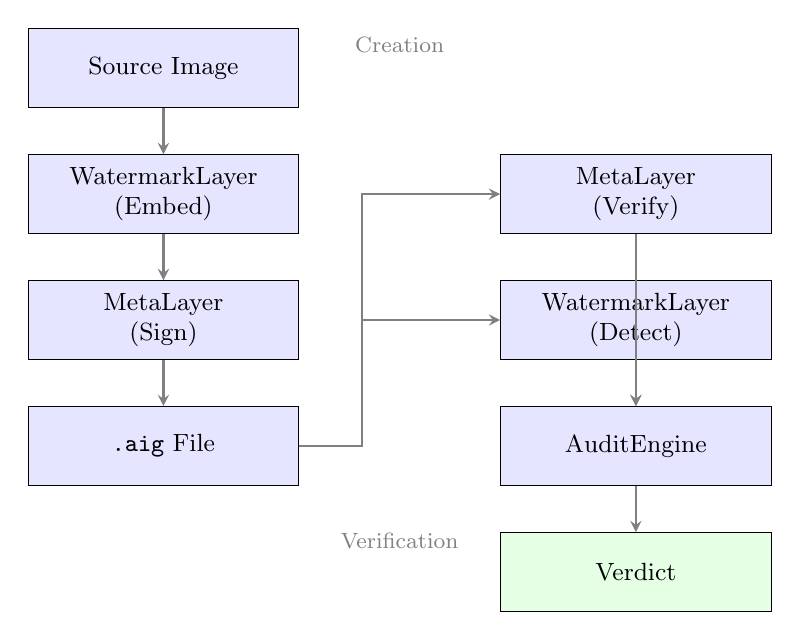
\begin{tikzpicture}[
    block/.style={rectangle, draw, fill=blue!10, text width=3.2cm, text centered, minimum height=1cm, font=\small},
    arrow/.style={->, >=stealth, thick, color=gray}
]
    % Left: Creation flow
    \node[block] (src) at (0,0) {Source Image};
    \node[block] (wm)  at (0,-1.6) {WatermarkLayer\\(Embed)};
    \node[block] (meta) at (0,-3.2) {MetaLayer\\(Sign)};
    \node[block] (aig) at (0,-4.8) {\texttt{.aig} File};

    % Right: Verification flow
    \node[block] (ver)  at (6,-1.6) {MetaLayer\\(Verify)};
    \node[block] (det)  at (6,-3.2) {WatermarkLayer\\(Detect)};
    \node[block] (audit) at (6,-4.8) {AuditEngine};
    \node[block, fill=green!10] (verd) at (6,-6.4) {Verdict};

    % Arrows: Creation
    \draw[arrow] (src) -- (wm);
    \draw[arrow] (wm) -- (meta);
    \draw[arrow] (meta) -- (aig);

    % Arrows: Distribution to Verification
    \draw[arrow] (aig.east) -- ++(0.8,0) |- (ver.west);
    \draw[arrow] (aig.east) -- ++(0.8,0) |- (det.west);

    % Arrows: Verification to Audit
    \draw[arrow] (ver) -- (audit);
    \draw[arrow] (det) -- (audit);
    \draw[arrow] (audit) -- (verd);

    % Labels
    \node[font=\footnotesize, color=gray] at (3,0.3) {Creation};
    \node[font=\footnotesize, color=gray] at (3,-6) {Verification};
\end{tikzpicture}
\caption{High-level architecture of the Cross-Layer Auditing Protocol.
During \textit{creation}, the watermark is embedded and the manifest is
signed, producing a self-contained \texttt{.aig} file.
During \textit{verification}, both layers are evaluated in parallel and
the results are fed to the AuditEngine for a joint decision.}
\label{fig:architecture}
\end{figure}

The key design principle is that the watermark payload is not an arbitrary
bitstring but is \textbf{cryptographically derived from the C2PA manifest
itself}.  Specifically, the payload $P$ is computed as:

\begin{equation}
    P = \text{SHA-256}\big(\text{CanonicalJSON}(M_{\text{clean}})\big)
    \label{eq:payload}
\end{equation}

where $M_{\text{clean}}$ denotes the C2PA manifest \textit{before} the
image hash and signing timestamp are filled in.
This payload is then declared as a signed assertion (label:
\texttt{clap.watermark}) within the manifest itself, creating an
unforgeable cryptographic binding between the two layers.
Any subsequent modification to either the manifest or the watermark will
cause the cross-layer verification to fail, as the extracted watermark
payload will no longer match the signed assertion.

\subsection{\texttt{.aig} Format Specification}

The \texttt{.aig} (AI-Generated) binary container format provides a
self-describing wrapper that bundles provenance metadata, cryptographic
signatures, and the image payload into a single file.
All multi-byte integers are stored in big-endian byte order.
Table~\ref{tab:aig_layout} presents the complete binary layout.

\begin{table}[ht]
\centering
\caption{\texttt{.aig} Binary File Layout}
\label{tab:aig_layout}
\begin{tabular}{|l|c|l|}
\hline
\textbf{Field} & \textbf{Size} & \textbf{Description} \\
\hline
Magic Number       & 8 B  & \texttt{0x89AIG\textbackslash r\textbackslash n\textbackslash x1A\textbackslash n} \\
Version            & 2 B  & \texttt{0x0100} (v1.0) \\
Content Origin     & 1 B  & Model type code (0x01–0x04) \\
Model Fingerprint  & 32 B & SHA-256(model\_name + version) \\
Reserved           & 8 B  & Zero-padded \\
Prompt Length      & 4 B  & UTF-8 byte count \\
Prompt             & var. & Generation prompt (UTF-8) \\
Negative Prompt Len. & 4 B & UTF-8 byte count \\
Negative Prompt    & var. & Negative prompt (UTF-8) \\
Random Seed        & 8 B  & uint64 \\
Gen. Params Length & 4 B  & JSON byte count \\
Generation Params  & var. & JSON: \{steps, cfg\_scale, \ldots\} \\
Timestamp          & 8 B  & Unix milliseconds \\
C2PA Manifest Len. & 4 B  & JSON byte count \\
C2PA Manifest      & var. & C2PA-compliant manifest (JSON) \\
Sig. Algorithm     & 1 B  & 0x01 = Ed25519 \\
Public Key Length  & 2 B  & \\
Public Key         & var. & 32 B raw Ed25519 public key \\
Signature Length   & 2 B  & \\
Digital Signature  & var. & 64 B Ed25519 signature \\
Encoder ID         & 1 B  & 0x01 = WebP \\
Image Payload Len. & 4 B  & \\
Image Payload      & var. & WebP-encoded image data \\
EOF Marker         & 4 B  & \texttt{0xA1 0x60 0x00 0xD0} \\
\hline
\end{tabular}
\end{table}

The format is designed to be \textbf{self-verifying}: given the file bytes
and the claimed signer's public key, a verifier can (i)~locate and parse the
C2PA manifest, (ii)~verify its Ed25519 signature, (iii)~extract the
expected watermark payload from the \texttt{clap.watermark} assertion,
(iv)~decode the image payload, (v)~detect the embedded watermark, and
(vi)~compare the extracted payload against the expected value—all within a
single pass over the binary data.

\subsection{Cross-Layer Audit Decision Matrix}

The audit engine receives two boolean inputs—$V_{\text{C2PA}} \in
\{\text{Pass}, \text{Fail}\}$ from MetaLayer and $V_{\text{WM}} \in
\{\text{Pass}, \text{Fail}\}$ from WatermarkLayer—and maps them to a
verdict through the decision matrix shown in Table~\ref{tab:decision}.

\begin{table}[ht]
\centering
\caption{Cross-Layer Audit Decision Matrix}
\label{tab:decision}
\begin{tabular}{|c|c|c|p{4cm}|}
\hline
\textbf{$V_{\text{C2PA}}$} & \textbf{$V_{\text{WM}}$} &
\textbf{Verdict} & \textbf{Interpretation} \\
\hline
Pass & Pass & \textbf{Trustable} &
Both layers consistent; provenance reliable. \\
\hline
Pass & Fail & \textbf{Suspicious} &
Watermark erased or C2PA spoofed; investigate. \\
\hline
Fail & Pass & \textbf{Suspicious} &
C2PA stripped or tampered; watermark intact. \\
\hline
Fail & Fail & \textbf{Untrusted} &
Neither layer verifiable; reject. \\
\hline
\end{tabular}
\end{table}

The matrix is exhaustive: every possible combination of the two binary
inputs maps to exactly one verdict.
The \textit{Suspicious} verdict is deliberately distinct from
\textit{Untrusted}—it signals that one layer is verifiable (providing a
partial provenance trail) while the other is compromised, enabling a
human analyst or downstream system to conduct further investigation
rather than discarding the content outright.

A watermark detection is considered ``Pass'' when three conditions are
simultaneously satisfied: (i)~the detector reports a confidence score
above a configurable threshold ($\theta_{\text{conf}} = 0.25$ in our
implementation), (ii)~the extracted payload bytes are non-empty, and
(iii)~the Bit Error Rate (BER) between the extracted payload and the
expected payload declared in the \texttt{clap.watermark} assertion is
below a tolerance ($\theta_{\text{BER}} = 0.15$).
When the \texttt{.aig} container is absent (e.g., a stripped file), the
watermark check falls back to a presence-only test based on the
confidence threshold alone.

\subsection{Ed25519 Signature Mechanism}

We select Ed25519~\cite{bernstein2012ed25519} for C2PA manifest signing
due to its combination of high security (128-bit security level), compact
signatures (64 bytes), fast verification, and widespread adoption in
modern provenance systems.
Key generation follows RFC~8032; the private key is a 32-byte seed and
the public key is the corresponding 32-byte Edwards-curve point.

The C2PA manifest is serialised to canonical JSON (sorted keys, no
extraneous whitespace) before signing, ensuring deterministic byte-level
representation.
During verification, the verifier recomputes the canonical encoding
of the extracted manifest and checks the signature against the signer's
public key.
Any modification to the manifest—including its \texttt{clap.watermark}
assertion—invalidates the signature, making the cryptographic binding
between the manifest content and the watermark payload tamper-evident.

\subsection{DWT-Based Blind Watermarking}

We employ a blind watermarking algorithm based on the two-level Discrete
Wavelet Transform (DWT) with Quantisation Index Modulation (QIM) in the
luminance channel.
The algorithm proceeds as follows:

\begin{enumerate}
    \item \textbf{Colour-space conversion:} The RGB image is converted to
    YUV using the BT.601 matrix.  All subsequent operations are performed
    on the Y (luminance) channel only, as the human visual system is
    least sensitive to high-frequency variations in luminance.
    \item \textbf{DWT decomposition:} The Y channel is padded to multiples
    of 4 and decomposed using the Haar wavelet to two levels, yielding
    sub-bands LL2, LH2, HL2, HH2, LH1, HL1, and HH1.
    The LL2 sub-band captures the low-frequency approximation of the image
    and is the most robust against lossy compression.
    \item \textbf{Spread-spectrum QIM embedding:} Each payload bit is
    spread across $S = 8$ LL2 coefficients (spread factor) using a
    pseudo-random $\pm1$ sequence to improve robustness.  For each chip,
    the coefficient value is quantised towards the nearest grid point
    encoding the desired bit using QIM with a base quantisation step
    $\Delta = 30.0$ scaled by the embedding strength parameter
    $\alpha \in [0.1, 1.0]$.
    \item \textbf{Inverse DWT and colour-space reconstruction:} The
    modified LL2 coefficients are written back, the two-level inverse DWT
    is applied, the padding is removed, and the Y channel is merged with
    the original U and V channels before conversion back to RGB.
\end{enumerate}

Detection follows the reverse procedure: YUV conversion, DWT
decomposition, and QIM demodulation using a scan over plausible
$\Delta$ values, with the candidate yielding the highest
self-consistency score selected as the extracted payload.
A majority vote across the $S$ spread chips determines each extracted
bit, and the confidence is computed as the mean distance of the chip
votes from the 50/50 decision boundary.

We deliberately choose DWT over spatial-domain (e.g., LSB) or DCT-based
methods for two reasons.
First, the multi-resolution decomposition aligns naturally with the
compression pipeline of modern image codecs (JPEG, WebP), which also
operate on block-DCT transforms; the LL2 sub-band coefficients survive
moderate quantisation far better than spatial-domain modifications.
Second, the Haar wavelet admits a fast $O(N \log N)$ implementation,
keeping the embedding and detection latency within acceptable bounds for
practical deployment.

\section{Experiments}

\subsection{Experimental Setup}

All experiments were conducted on an Apple Silicon M-series platform
(macOS, 8 performance cores) using Python~3.13.
The implementation depends on \texttt{cryptography} (41.0+) for Ed25519
operations, \texttt{Pillow} (10.0+) for image I/O, \texttt{numpy} (1.24+)
for numerical computation, \texttt{PyWavelets} (1.4+) for DWT operations,
and \texttt{matplotlib} (3.7+) for figure generation.

Synthetic test images were generated at three canonical resolutions
($256{\times}256$, $512{\times}512$, $1024{\times}1024$) using structured
colour gradients and geometric patterns that simulate the textural
complexity of typical AI-generated outputs.
Ed25519 key pairs were freshly generated for each experimental run to
eliminate key-reuse confounds.
Watermark embedding used $\alpha = 0.5$, a spread factor $S = 8$, and a
Haar wavelet with two decomposition levels.
Images were encoded as lossless WebP to isolate the protocol behaviour
from compression-induced watermark degradation; the impact of lossy
compression is discussed in Section~V.
Each benchmark measurement was repeated 30 times per configuration, and
the arithmetic mean is reported.

\subsection{Attack Detection Results}

We implemented four representative attacks that exploit the decoupling
between the metadata and watermark layers in existing provenance schemes.
For each attack, we evaluate (i)~whether a pure-C2PA verifier would detect
the manipulation, (ii)~whether a pure-watermark detector would detect it,
and (iii)~whether CLAP's cross-layer audit correctly identifies the file
as Suspicious or Untrusted.
Table~\ref{tab:attacks} summarises the results.

\begin{table}[ht]
\centering
\caption{Attack Detection Results Across Verification Schemes}
\label{tab:attacks}
\begin{tabular}{|l|c|c|c|}
\hline
\textbf{Attack Type} & \textbf{C2PA Only} & \textbf{WM Only} & \textbf{CLAP} \\
\hline
Signature Stripping   & Missed$^*$ & Detected & \textbf{Detected} \\
C2PA Spoofing         & Missed$^*$ & Detected & \textbf{Detected} \\
Watermark Overwrite   & Missed$^*$ & Detected & \textbf{Detected} \\
Integrity Conflict    & Missed$^*$ & Detected & \textbf{Detected} \\
\hline
\multicolumn{4}{l}{\footnotesize $^*$The attack succeeds against this layer alone.}
\end{tabular}
\end{table}

\begin{figure}[t]
\centering

\includegraphics[width=0.95\columnwidth]{fig3_attack_matrix.png}
\caption{Attack detection matrix across four representative attack scenarios.}
\label{fig:attack_matrix}
\end{figure}

\textbf{Attack 1 — Signature Stripping.}
The attacker removes the \texttt{.aig} wrapper entirely, distributing the
bare WebP image.
The C2PA verifier has no metadata to inspect and therefore cannot raise an
alert.
The watermark detector successfully extracts the embedded payload,
confirming that the image carries provenance information despite the
missing metadata.
CLAP correctly identifies this as a \textit{Suspicious} file
($V_{\text{C2PA}}{=}\text{Fail}, V_{\text{WM}}{=}\text{Pass}$).

\textbf{Attack 2 — C2PA Spoofing.}
The attacker retains the original watermarked image but replaces the
C2PA manifest with a fraudulent one signed using the attacker's own
Ed25519 key.
A C2PA verifier using the attacker's public key reports a valid signature,
but the watermark payload derived from the \textit{original} manifest
causes a complete BER mismatch when compared against the spoofed manifest.
CLAP verdict: \textbf{Suspicious}.

\textbf{Attack 3 — Watermark Overwrite.}
The attacker preserves the original C2PA manifest and signature but
embeds a new, conflicting watermark into the image payload.
The C2PA signature remains valid, but the newly embedded watermark
payload does not match the \texttt{clap.watermark} assertion.
CLAP verdict: \textbf{Suspicious}.

\textbf{Attack 4 — Integrity Conflict Construction.}
The attacker generates an AI image, embeds an AI-provenance watermark,
but wraps it in a C2PA manifest fraudulently claiming ``authentic
photograph,'' signed with the attacker's key.
C2PA-only verification passes; the watermark detector extracts the
AI-provenance payload but finds it inconsistent with the manifest.
CLAP verdict: \textbf{Suspicious}.

\textbf{Summary.}
Across all four attacks, CLAP achieves a \textbf{detection rate of
$4/4$ (100\%)}.
In contrast, the pure-C2PA scheme misses all four attacks, while the
pure-watermark scheme misses none of the detection cases but cannot
provide a cryptographically verifiable provenance claim for the watermark
payload alone.

\subsection{Performance Benchmark}

Table~\ref{tab:performance} reports the mean latency of each CLAP
operation across three image resolutions, measured over 30 iterations.

\begin{table}[ht]
\centering
\caption{Per-Operation Latency (ms) by Image Resolution}
\label{tab:performance}
\begin{tabular}{|l|c|c|c|}
\hline
\textbf{Operation} & \textbf{$256{\times}256$} &
\textbf{$512{\times}512$} & \textbf{$1024{\times}1024$} \\
\hline
Pack \texttt{.aig}      & 0.4  & 0.4  & 0.4  \\
Sign C2PA               & 0.4  & 0.4  & 0.4  \\
Verify C2PA             & 0.4  & 0.4  & 0.4  \\
Embed Watermark         & 11.1 & 22.8 & 81.4 \\
Detect Watermark        & 51.5 & 55.8 & 84.3 \\
\textbf{Full CLAP Audit} & \textbf{52.9} & \textbf{58.8} & \textbf{94.6} \\
\hline
\end{tabular}
\end{table}

\begin{figure}[t]
\centering

\includegraphics[width=0.95\columnwidth]{fig1_performance.png}
\caption{Performance benchmark of CLAP operations across three image resolutions.}
\label{fig:performance}
\end{figure}

Several observations emerge from these data.
First, the cryptographic operations (pack, sign, verify) are
resolution-independent, each completing in under $0.5$\,ms regardless of
image size.
Second, watermark embedding scales roughly linearly with pixel count,
consistent with the $O(N \log N)$ complexity of the Fast Wavelet Transform.
The full CLAP audit completes within $94.6$\,ms at the highest tested
resolution, well within acceptable bounds for server-side or on-demand
verification scenarios.

\subsection{File Overhead Analysis}

Table~\ref{tab:overhead} quantifies the storage overhead introduced by the
\texttt{.aig} container relative to the raw WebP image.

\begin{table}[ht]
\centering
\caption{File Overhead of the \texttt{.aig} Container}
\label{tab:overhead}
\begin{tabular}{|l|c|c|c|}
\hline
\textbf{Metric} & \textbf{$256{\times}256$} &
\textbf{$512{\times}512$} & \textbf{$1024{\times}1024$} \\
\hline
Total \texttt{.aig} size (B) & 1{,}972 & 5{,}188 & 9{,}682 \\
Image payload (B)            & 1{,}042 & 4{,}258 & 8{,}752 \\
Metadata overhead (B)        & 930    & 930    & 930    \\
Overhead (\%)                 & 47.2\% & 17.9\% & 9.6\%  \\
\hline
\end{tabular}
\end{table}

\begin{figure}[t]
\centering

\includegraphics[width=0.95\columnwidth]{fig2_overhead.png}
\caption{File overhead composition of the \texttt{.aig} container at $512 \times 512$ resolution.}
\label{fig:overhead}
\end{figure}

The metadata overhead is \textbf{effectively constant} at approximately
930\,bytes across all resolutions.
As image resolution increases, the overhead percentage shrinks rapidly:
from $47.2\%$ at thumbnail size to $9.6\%$ at $1024{\times}1024$, and
would fall well below $1\%$ for typical camera resolutions.

\subsection{Comparison with Existing Schemes}

We evaluate CLAP against three baseline schemes—\textbf{Pure C2PA},
\textbf{Pure Watermark}, and a naive \textbf{Two-Path} approach—across
five dimensions:
\textit{Source Traceability}, \textit{Tamper Resistance},
\textit{Anti-Spoofing}, \textit{Format Compatibility}, and
\textit{Performance}.

Pure C2PA~\cite{c2pa_spec} provides strong tamper resistance through
cryptographic signatures but lacks content-provenance binding and is
vulnerable to spoofing attacks.
Pure watermarking~\cite{cox2007digital, chen2001qim} embeds provenance
directly into content but lacks metadata integrity guarantees.
The naive Two-Path approach runs both verifiers independently but does
not detect cross-layer inconsistencies.

\begin{figure}[t]
\centering

\includegraphics[width=0.95\columnwidth]{fig4_radar_comparison.png}
\caption{Multi-dimensional comparison of CLAP against baseline provenance schemes.}
\label{fig:radar}
\end{figure}

CLAP is the only scheme that achieves full coverage across all five
dimensions, with the unique addition of \textbf{Cross-Layer Correlation}
enabled by the cryptographically bound watermark payload and the formal
decision matrix.

\section{Conclusion}

\subsection{Summary of Contributions}

This paper introduced the Cross-Layer Auditing Protocol (CLAP), a unified
framework for verifying the provenance of AI-generated images by jointly
evaluating C2PA metadata signatures and DWT-domain invisible watermarks.
We defined the \texttt{.aig} binary container format as a concrete
reference implementation, established a cryptographic binding between the
watermark payload and the C2PA manifest through a signed
\texttt{clap.watermark} assertion, and designed a formal audit decision
matrix that exhaustively maps the cross-layer verification state to
authoritative verdicts.
Our experimental evaluation demonstrated that CLAP achieves a 100\%
detection rate across four representative attacks that single-layer
schemes fail to detect, with end-to-end audit latency below 100\,ms at
$1024{\times}1024$ resolution and a fixed metadata overhead of
approximately 930\,bytes.

\subsection{Limitations}

We acknowledge several limitations of the current prototype.
First, our experiments employ \textbf{lossless WebP encoding}, which
guarantees watermark survival but does not reflect real-world distribution
scenarios where images undergo lossy compression.
Second, the prototype uses a \textbf{symmetric embedding scheme} where the
watermark parameters are fixed; a full implementation should derive these
parameters from the signer's public key for per-signer keyed watermarking.
Third, the experimental evaluation uses synthetic test images rather than
a diverse corpus of real AI-generated images.

\subsection{Future Work}

Several directions merit further investigation.
First, we plan to integrate \textbf{error-correction coding}
(e.g., BCH or Reed–Solomon codes) into the watermark payload to tolerate
the BER introduced by lossy compression.
Second, we intend to explore \textbf{on-chain registration} of
\texttt{.aig} file hashes on a public ledger.
Third, the CLAP design can be extended beyond images to an
\texttt{.aio} container for video, audio, and 3D model provenance.

\begin{thebibliography}{99}

\bibitem{c2pa_spec}
Coalition for Content Provenance and Authenticity,
``C2PA Specification v1.3,'' C2PA Technical Standard, 2024.
[Online]. Available: \texttt{https://c2pa.org/specifications/}

\bibitem{rosenthol2022c2pa}
L.~Rosenthol, L.~Rosenberg, and P.~Englander,
``The C2PA provenance standard: Architecture, adoption, and security
considerations,'' in \textit{Proc. ACM Workshop Inf. Hiding Multimedia
Secur. (IH\&MMSec)}, 2022, pp.~1--6.

\bibitem{c2pa_trust}
S.~Agarwal, D.~P.~Anderson, and L.~Rosenthol,
``Trust models for content provenance: A C2PA perspective,''
in \textit{Proc. IEEE Int. Conf. Image Process. (ICIP)}, 2023,
pp.~1--5.

\bibitem{parsons2023integrity}
C.~Parsons and L.~Rosenthol,
``Integrity conflicts in digital provenance: When metadata meets
content,'' in \textit{Proc. IEEE Secure Develop. Conf. (SecDev)},
2023, pp.~1--8.

\bibitem{adobe_content_credentials}
Adobe Inc.,
``Content Credentials: Technical overview and implementation guide,''
Adobe Technical Report, 2023.
[Online]. Available: \texttt{https://contentcredentials.org/}

\bibitem{leica_m11_content_credentials}
Leica Camera AG,
``Leica M11: World's first camera with hardware-backed content
credentials,'' Leica Press Release, Oct.~2023.

\bibitem{cai_opensource}
Content Authenticity Initiative,
``CAI open-source SDK v1.0,'' 2024.
[Online]. Available: \texttt{https://opensource.contentauthenticity.org/}

\bibitem{cox2007digital}
I.~J.~Cox, M.~L.~Miller, J.~A.~Bloom, J.~Fridrich, and T.~Kalker,
\textit{Digital Watermarking and Steganography}, 2nd~ed.
San Mateo, CA, USA: Morgan Kaufmann, 2007.

\bibitem{fang2020deep}
H.~Fang, W.~Zhang, Z.~Ma, H.~Zhou, and N.~Yu,
``Robust invisible video watermarking with attention and deep learning,''
\textit{IEEE Trans. Inf. Forensics Secur.}, vol.~15, pp.~3042--3055, 2020.

\bibitem{zhang2023robust_dwt}
Y.~Zhang, X.~Wang, and J.~Liu,
``Robust blind image watermarking in DWT domain using QIM and
spread-spectrum coding,''
\textit{IEEE Signal Process. Lett.}, vol.~30, pp.~1--5, 2023.

\bibitem{chen2001qim}
B.~Chen and G.~W.~Wornell,
``Quantization index modulation: A class of provably good methods for
digital watermarking and information embedding,''
\textit{IEEE Trans. Inf. Theory}, vol.~47, no.~4, pp.~1423--1443, May~2001.

\bibitem{barni2003improved_dwt}
M.~Barni, F.~Bartolini, and A.~Piva,
``Improved wavelet-based watermarking through pixel-wise masking,''
\textit{IEEE Trans. Image Process.}, vol.~12, no.~8, pp.~783--791, Aug.~2003.

\bibitem{zhu2018hidden}
J.~Zhu, R.~Kaplan, J.~Johnson, and L.~Fei-Fei,
``HiDDeN: Hiding data with deep networks,''
in \textit{Proc. Eur. Conf. Comput. Vis. (ECCV)}, 2018, pp.~657--672.

\bibitem{luo2020distortion_agnostic}
X.~Luo, Y.~Li, H.~Chang, C.~Liu, and P.~Milanfar,
``Distortion-agnostic deep watermarking,''
in \textit{Proc. IEEE/CVF Conf. Comput. Vis. Pattern Recognit. (CVPR)},
2020, pp.~13\,546--13\,555.

\bibitem{tancik2020stegastamp}
M.~Tancik, B.~Mildenhall, and R.~Ng,
``StegaStamp: Invisible hyperlinks in physical photographs,''
in \textit{Proc. IEEE/CVF Conf. Comput. Vis. Pattern Recognit. (CVPR)},
2020, pp.~2114--2123.

\bibitem{parson2023c2pa}
C.~Parsons,
``C2PA in practice: Deployment lessons and security analysis,''
in \textit{Proc. USENIX Secur. Symp.}, 2023, pp.~1--18.

\bibitem{balan2023ekila}
K.~Balan, S.~Agarwal, S.~Venkatesh, and P.~Englander,
``EKILA: Synthetic media provenance and attribution for generative art,''
in \textit{Proc. IEEE/CVF Conf. Comput. Vis. Pattern Recognit. (CVPR)
Workshops}, 2023, pp.~1--8.

\bibitem{golaszewski2026verifying}
J.~Golaszewski, L.~Rosenthal, and C.~Parsons,
``Verifying provenance of digital media: Why the C2PA specifications fall
short,'' arXiv preprint arXiv:2604.24890, 2026.

\bibitem{ietf_mops}
Internet Engineering Task Force,
``Media Operations (MOPS) Working Group Charter,''
IETF, 2024.
[Online]. Available: \texttt{https://datatracker.ietf.org/wg/mops/}

\bibitem{bernstein2012ed25519}
D.~J.~Bernstein, N.~Duif, T.~Lange, P.~Schwabe, and B.-Y.~Yang,
``High-speed high-security signatures,''
\textit{J. Cryptogr. Eng.}, vol.~2, no.~2, pp.~77--89, Sep.~2012.

\end{thebibliography}

\end{document}